\documentclass[a4paper,12pt]{article}
\usepackage[utf8]{inputenc}
\usepackage[T1]{fontenc}
\usepackage[french]{babel}
\usepackage{geometry}
\usepackage{graphicx}
\geometry{margin=2.5cm}

% En-têtes et pieds de page
\usepackage{fancyhdr}
\pagestyle{fancy}
\fancyhf{}
\fancyhead[L]{Portfolio WordPress}
\fancyhead[R]{Mignard Mael}
\fancyfoot[C]{\thepage}

\title{Résumé et Rapport sur la création d’un portfolio WordPress}
\author{Mignard Mael}
\date{\today}

\begin{document}

\maketitle
\tableofcontents

\section*{Introduction}
Ce document résume les étapes de création d’un portfolio WordPress en local 
avec MAMP et fournit des explications sur certaines notions techniques : 
adresse \texttt{127.0.0.1}, modèle client/serveur, et rôle du backend PHP/MySQL. 
Le site est accessible en local via \texttt{http://127.0.0.1/monportfolio}.

\section{Résumé des grandes étapes}

\subsection*{Installation et configuration}
\begin{itemize}
    \item Installer MAMP et démarrer Apache + MySQL.
    \item Créer une base de données via phpMyAdmin (ex. \texttt{portfolio\_wp}).
\end{itemize}

\subsection*{Installation de WordPress}
\begin{itemize}
    \item Télécharger WordPress et placer le dossier dans \texttt{htdocs}.
    \item Lancer l’installation via \texttt{http://localhost:8888/monportfolio}.
\end{itemize}

\subsection*{Configuration et pages principales}
\begin{itemize}
    \item Se connecter au tableau de bord WordPress.
    \item Installer un thème adapté au portfolio.
    \item Définir la page d’accueil statique et la page des articles.
    \item Créer les pages : Accueil, À propos, Portfolio, Contact, Blog (optionnel).
\end{itemize}

\subsection*{Menu et contenu}
\begin{itemize}
    \item Créer et organiser le menu principal pour accéder à toutes les pages.
    \item Ajouter les articles, projets et fichiers téléchargeables.
\end{itemize}

\subsection*{Personnalisation et rendu}
\begin{itemize}
    \item Personnaliser couleurs, polices, logo et images.
    \item Vérifier le fonctionnement de toutes les pages et liens.
    \item Préparer le rendu : zip du dossier WordPress + export SQL de la base.
\end{itemize}

\section{Explications théoriques}

\subsection*{Qu’est-ce que 127.0.0.1 ?}
127.0.0.1 est l’adresse IP de \textbf{loopback} (localhost). 
Elle permet d’accéder à un serveur qui tourne en local sur son propre ordinateur. 
C’est une adresse spéciale qui redirige toujours vers la machine sur laquelle on travaille.

\subsection*{Modèle client / serveur}
Le fonctionnement de WordPress repose sur le modèle \textbf{client/serveur} :
\begin{itemize}
    \item Le \textbf{client} est le navigateur web (Chrome, Firefox…) qui envoie une requête 
    pour afficher une page.
    \item Le \textbf{serveur} est Apache (via MAMP) qui reçoit la requête et renvoie la page web.
\end{itemize}
La communication se fait via le protocole HTTP. Dans ce projet, client et serveur 
sont sur le même ordinateur, d’où l’usage de 127.0.0.1.

\subsection*{Rôle du backend (PHP + MySQL)}
\begin{itemize}
    \item \textbf{PHP} : langage exécuté côté serveur, qui génère les pages dynamiques.
    \item \textbf{MySQL} : base de données qui stocke le contenu du site (pages, articles, utilisateurs, réglages).
\end{itemize}
Lorsqu’une page WordPress est ouverte, le serveur Apache exécute le code PHP, 
qui interroge MySQL pour récupérer les informations, puis renvoie le résultat en HTML/CSS 
au navigateur.


\clearpage
\section*{Captures d'écrans}

\begin{figure}[h!]
    \centering
    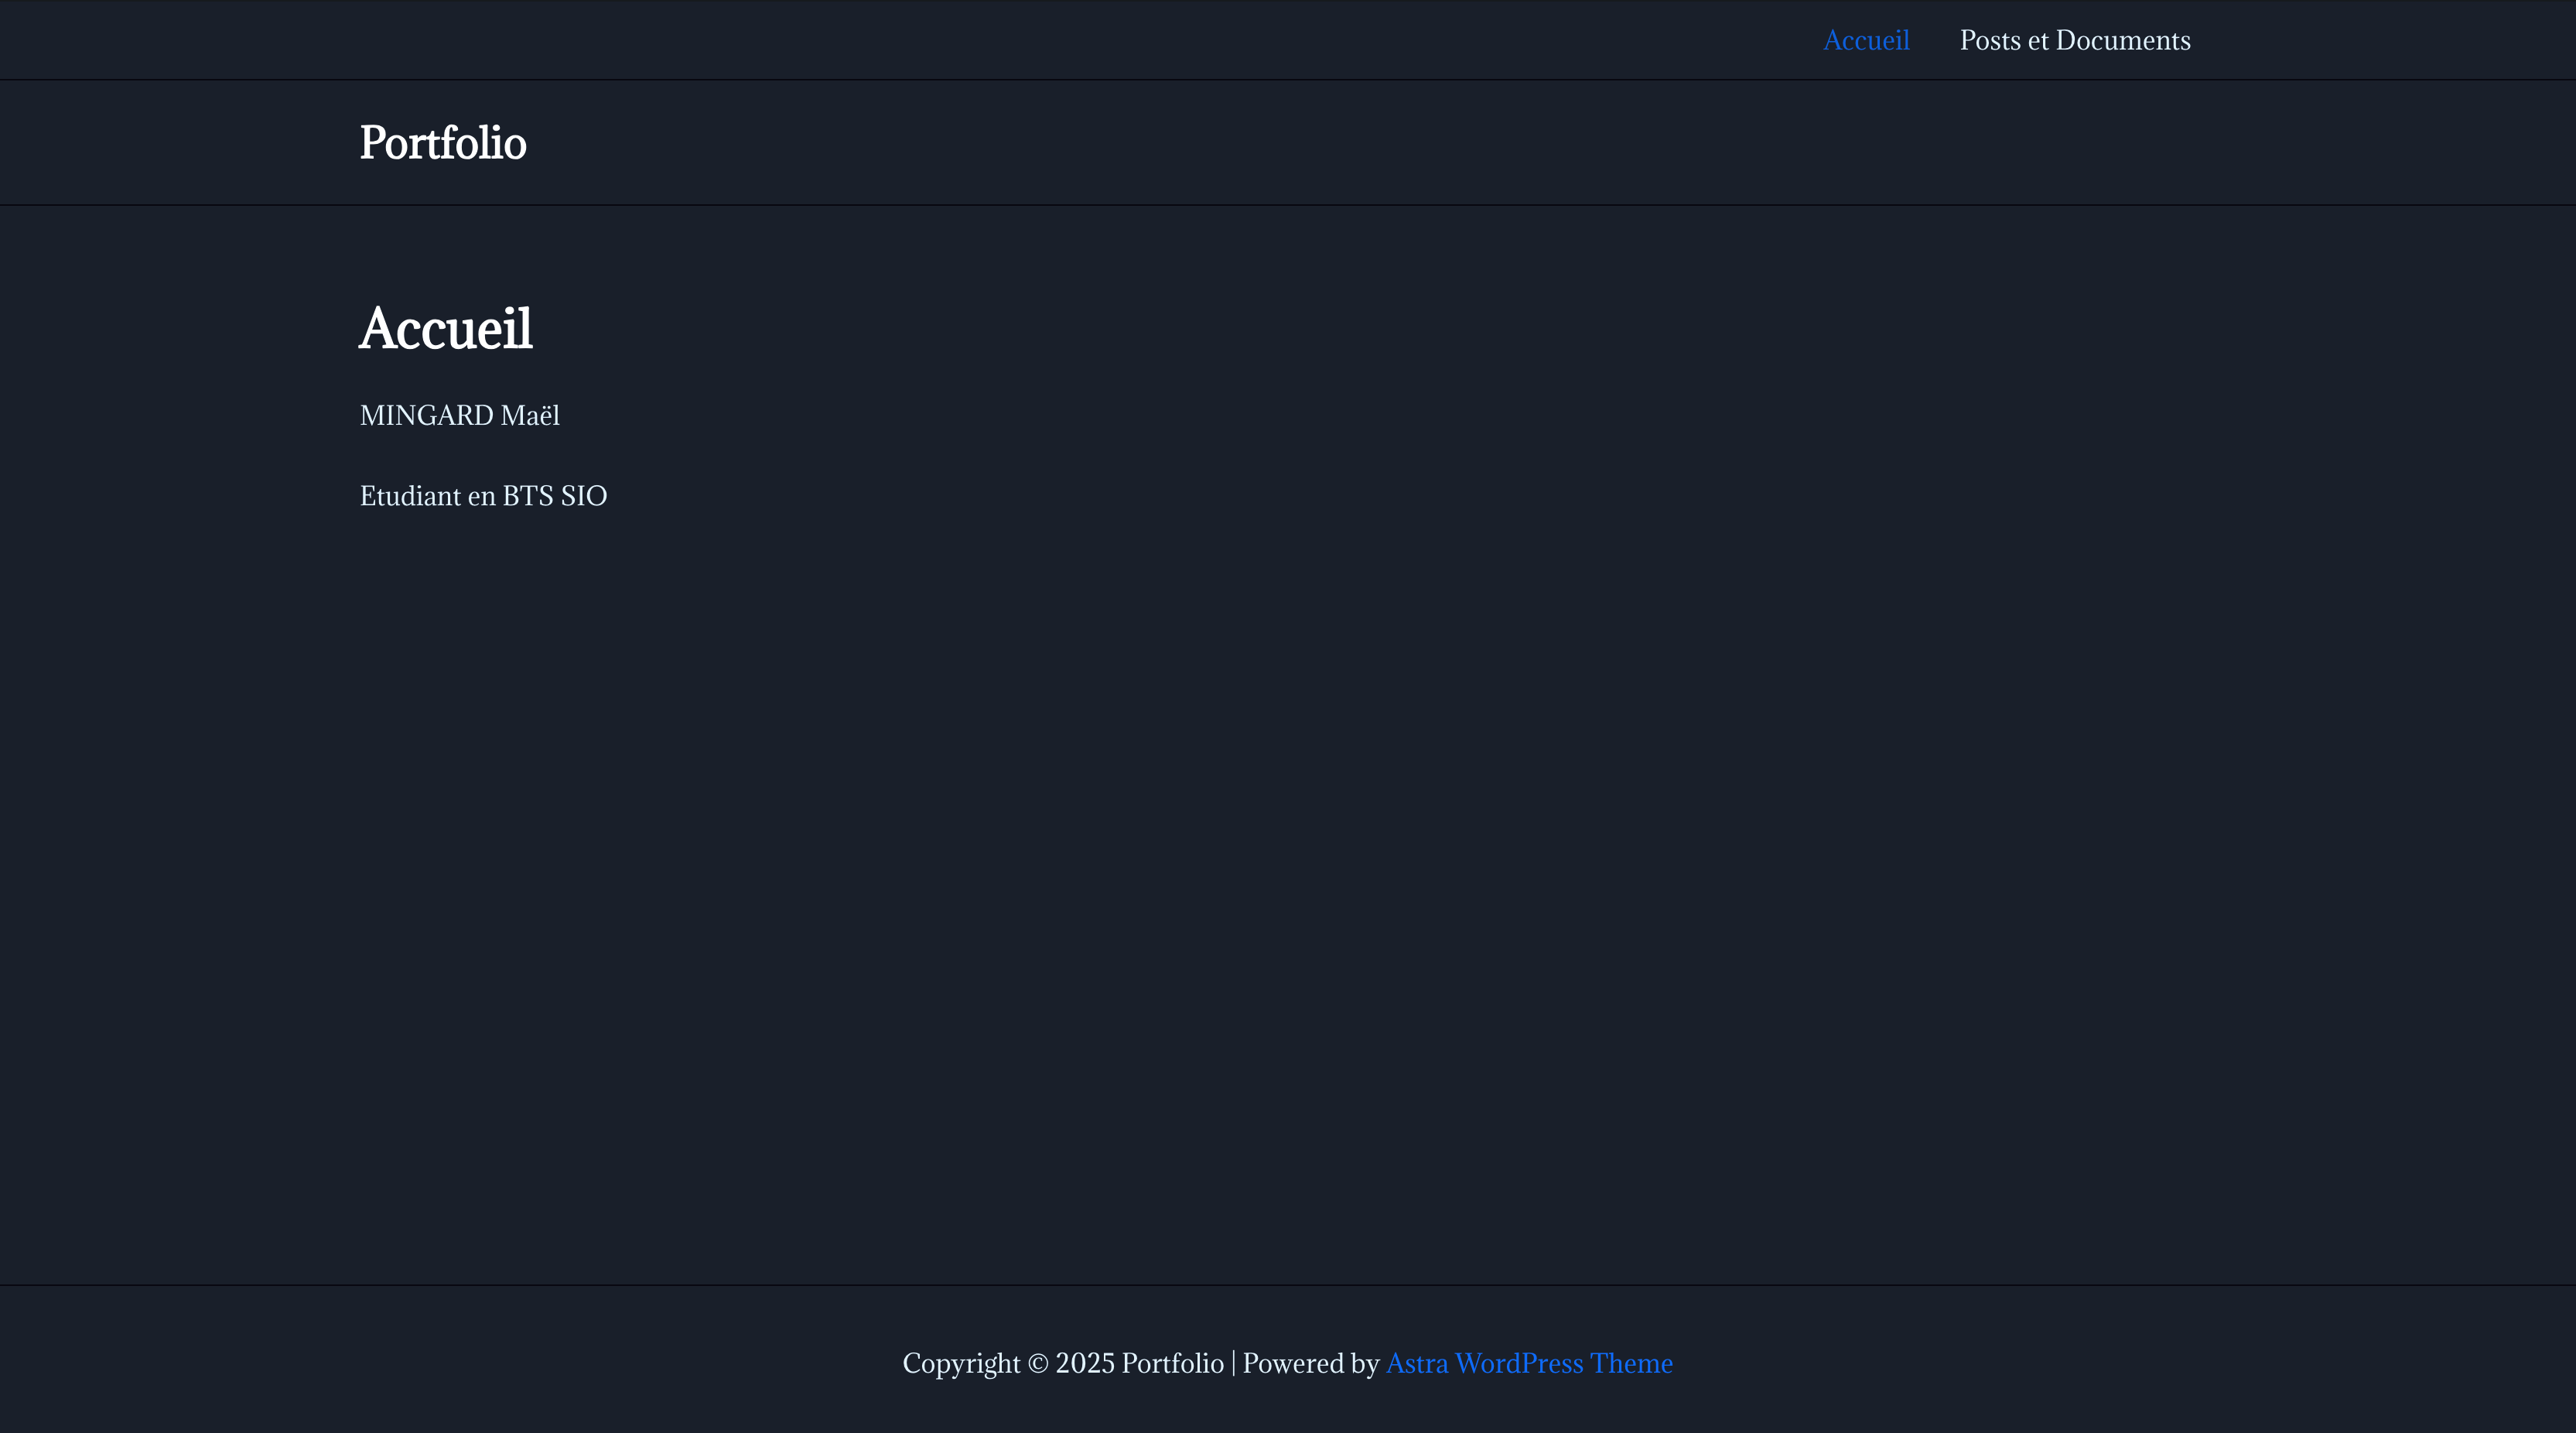
\includegraphics[width=0.8\textwidth]{home.png}
    \caption{Page d'accueil}
    \label{fig:capture1}
\end{figure}

\begin{figure}[h!]
    \centering
    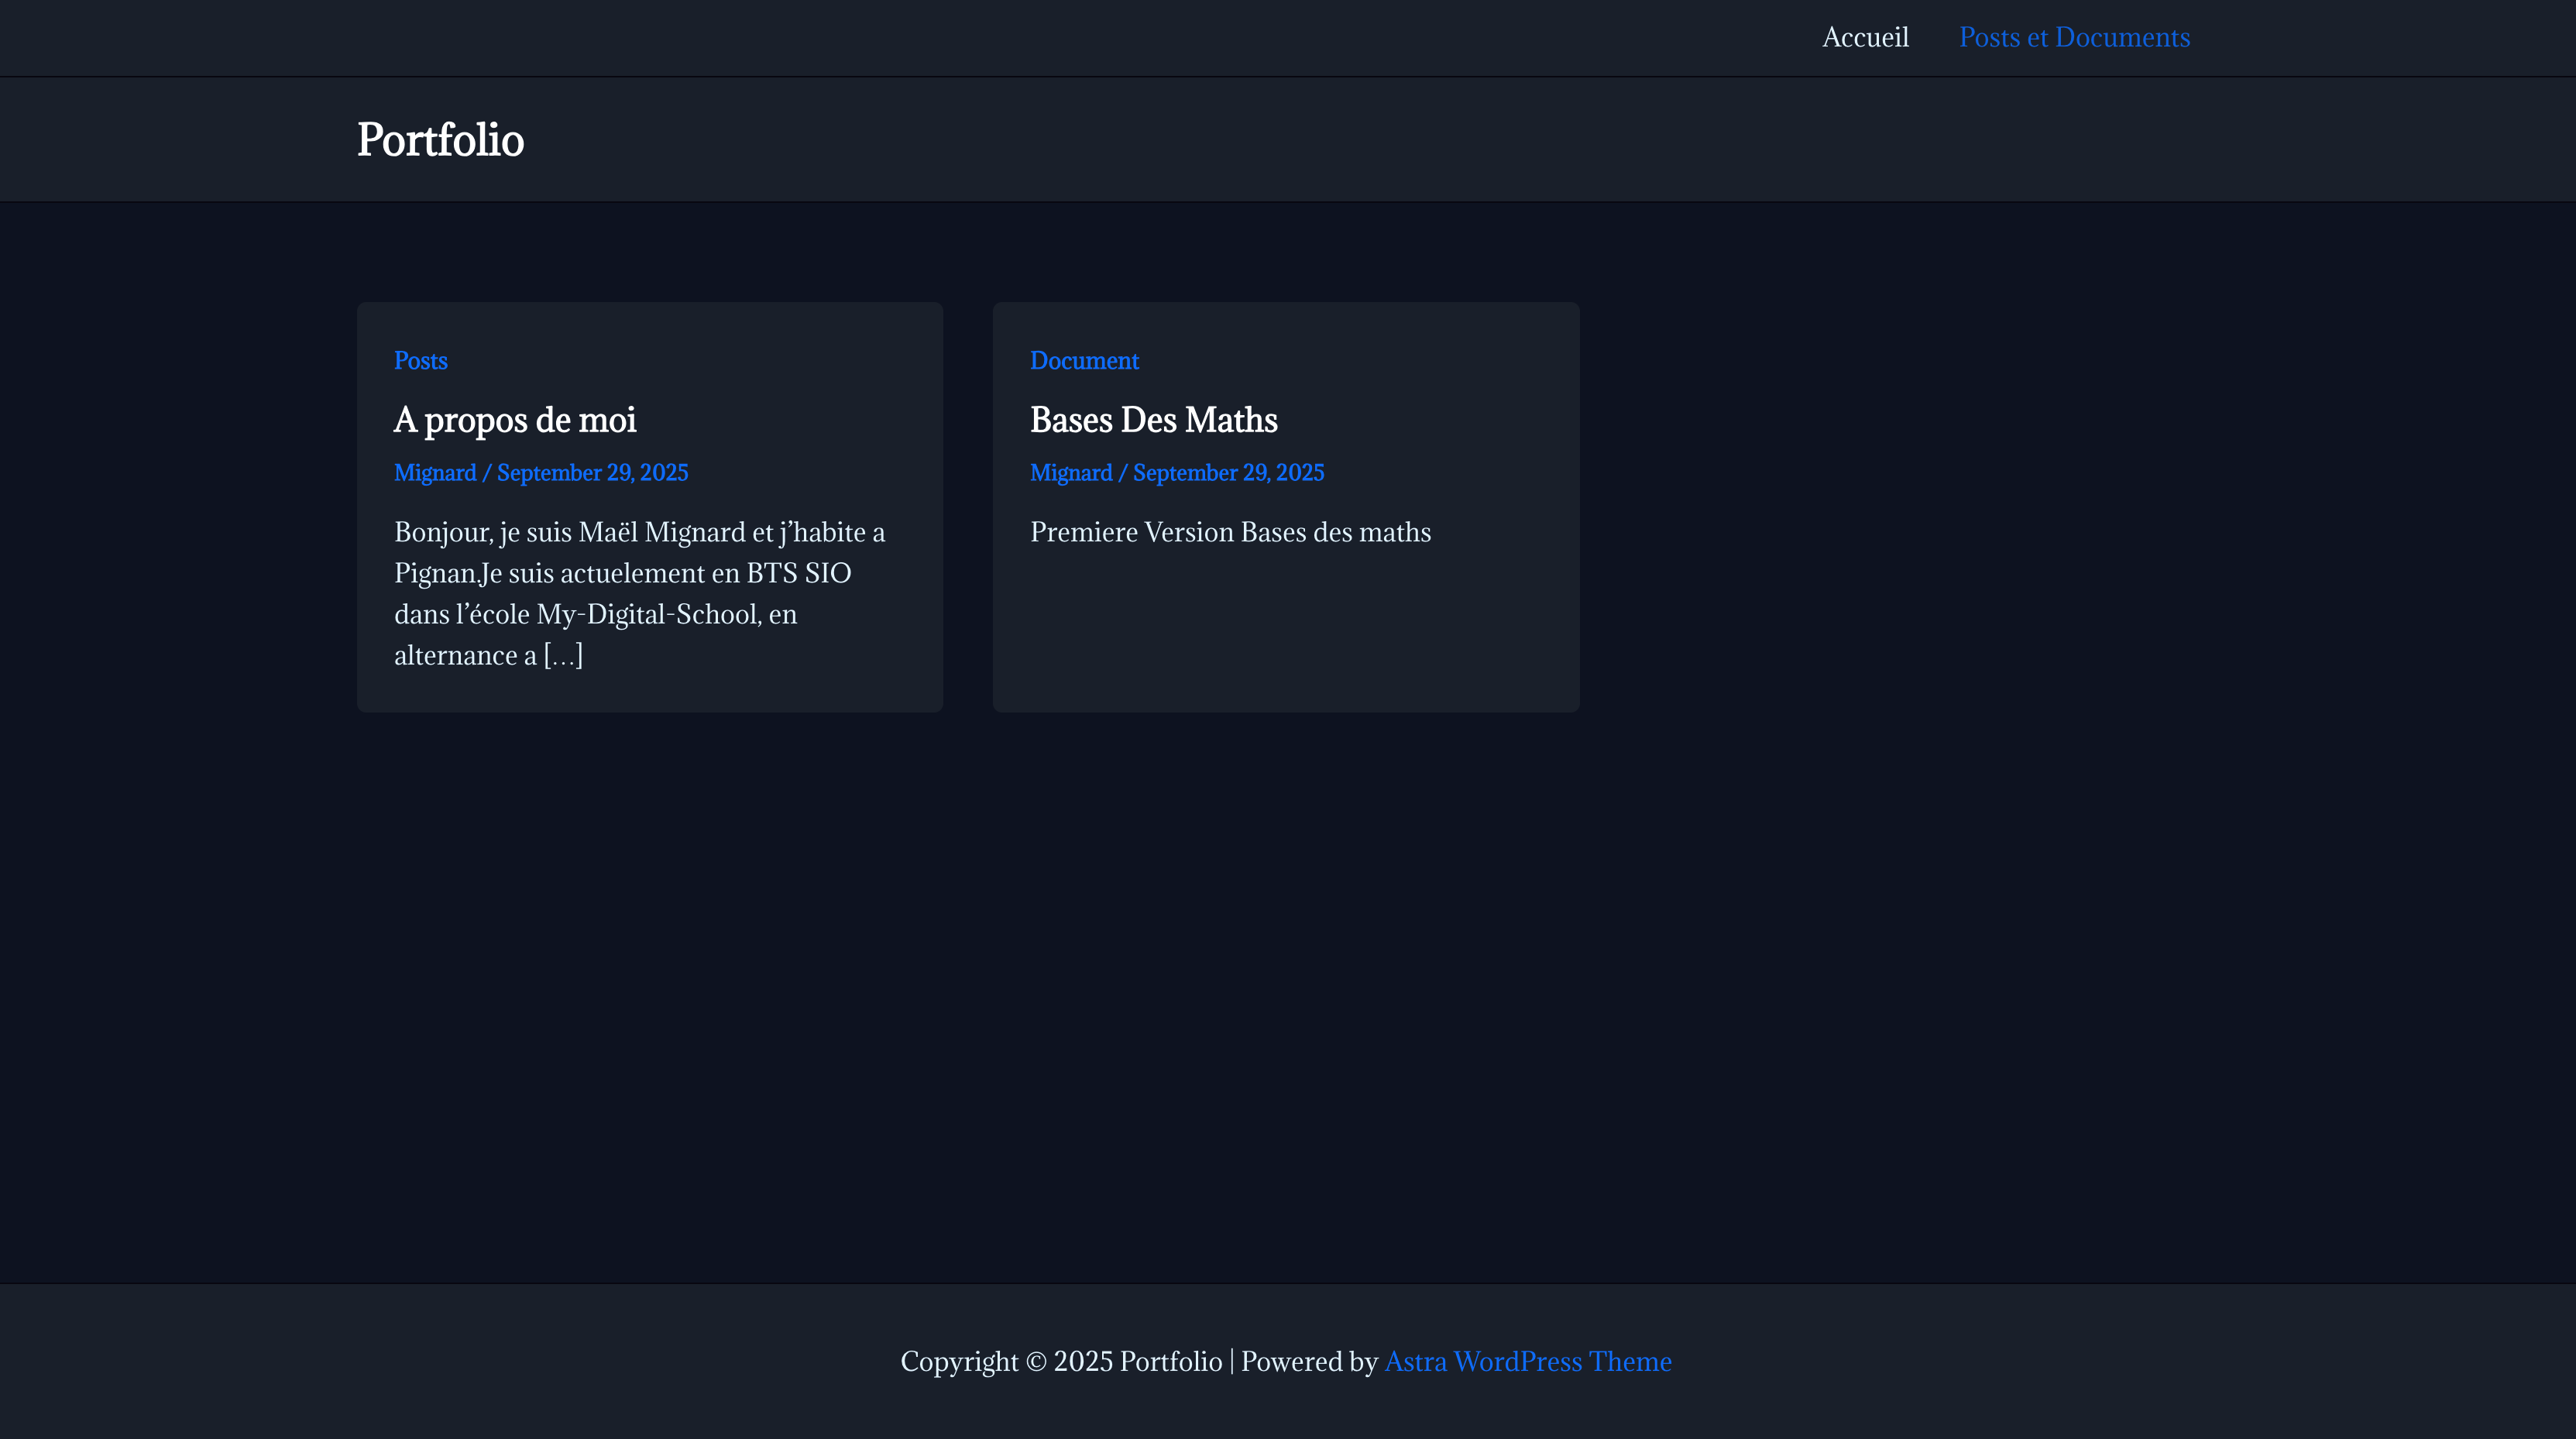
\includegraphics[width=0.8\textwidth]{post.png}
    \caption{Page des Post et Documents}
    \label{fig:capture2}
\end{figure}

\end{document}
